% Defines the document class
\documentclass[10pt,portuguese]{beamer}

% Defines the theme
\usetheme{metropolis}

% Imports the pre-defined packages
\usepackage{styles/packages}

% Imports the pre-defined templates
\usepackage{styles/templates}

% Imports the pre-defined colors
\usepackage{styles/colors}

% Imports the first slide's header
\usepackage{styles/header}

% Defines meta-information about the presentation
\title{Ampliando a Visibilidade de Pesquisas através de Códigos Abertos e Repositórios Oficiais}
\subtitle{\emph{X Workshop do Programa de Pós-Graduação em Ciência da Computação}}
\date{\today}
\author{Gustavo de Rosa}
\institute{
    Universidade Estadual Paulista ``Júlio de Mesquita Filho" (UNESP)
    \\
    Faculdade de Ciências (FC) / Departamento de Computação (DCo)
    \\
    Bauru, SP - Brasil
}

% Finishes up the preamble definition and starts the document
\begin{document}

% Makes up the preamble slide
\maketitle

% Imports the corresponding slides
\begin{frame}{Sumário da apresentação}
    \tableofcontents[sections={1-3}]
\end{frame}

\begin{frame}{}
    \tableofcontents[sections={4-6}]
\end{frame}
\section{Introdução}
\label{s.introduction}

\begin{frame}{Introdução}
	\vspace{0.4cm}
	\justify A área de Ciência da Computação sempre está evoluindo, onde diariamente dezenas de artigos novos estão disponíveis, e.g., \url{https://arxiv.org};
	\\~\\
	\begin{figure}
		\centering
		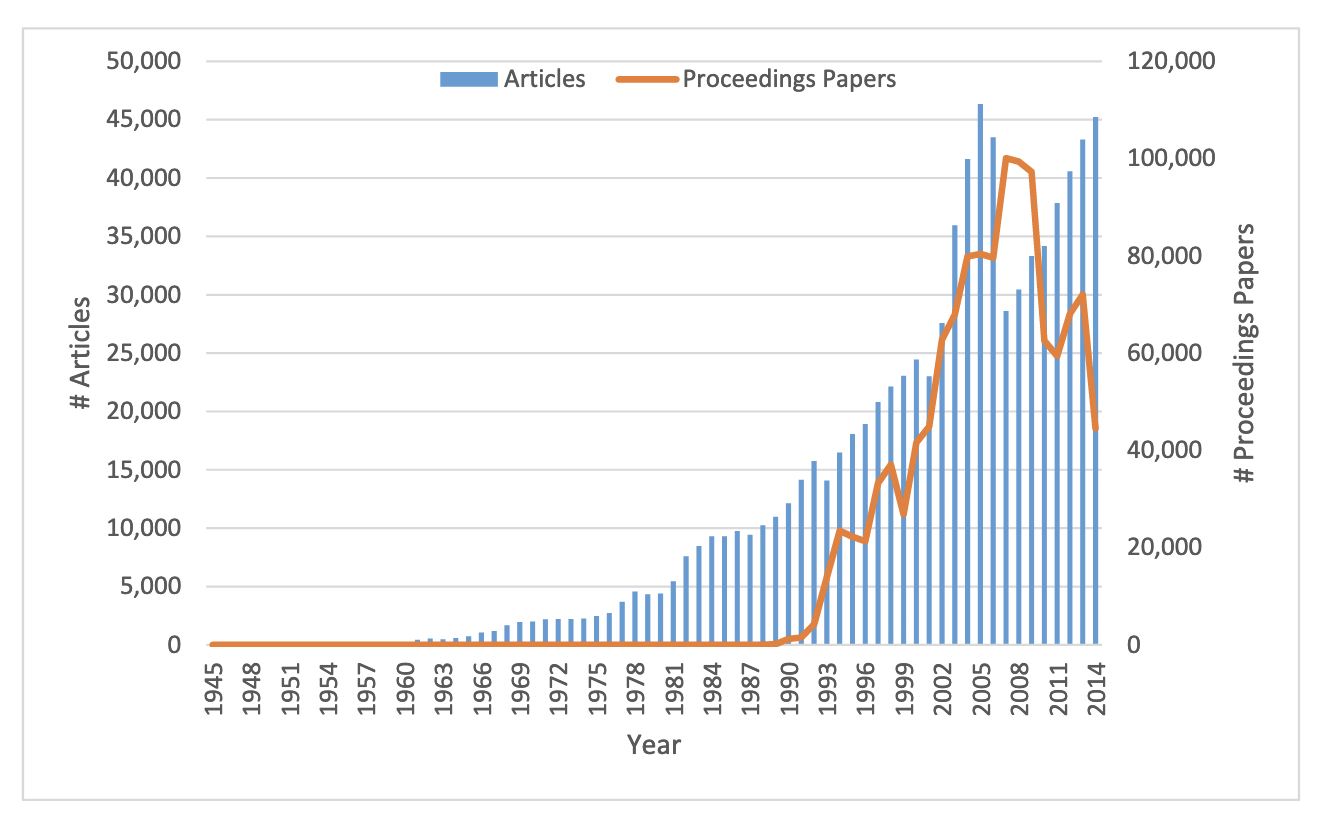
\includegraphics[scale=0.3]{figs/number_of_papers.png}
		\caption{Número de artigos (periódicos em azul e conferências em laranja) publicados em anos individuais~\cite{Fiala:17}.}
	\end{figure}
\end{frame}

\begin{frame}{}
	\begin{columns}
		\begin{column}{0.5\textwidth}
			\justify Atualmente, centros de pesquisa privados estão ``competindo"~diretamente com as universidades;	
		\end{column}
		\begin{column}{0.5\textwidth}
			\begin{figure}
				\centering
				
\includegraphics[scale=0.6]{figs/private_company.png}
			\end{figure}	
		\end{column}
	\end{columns}

\end{frame}

\begin{frame}{}
	\justify Entretanto, como é possível garantir a \textbf{visibilidade} da pesquisa em um mundo altamente competitivo?
\end{frame}
\section{Visibilidade}
\label{s.visibility}

\subsection{O que é?}
\label{ss.what_visibility}

\begin{frame}{O que é?}
	\justify 
	\begin{itemize}
		\item<1> Do latim \textit{visibilitas}, visibilidade é a qualidade/estado do que é visível;
		\\~\\
		\item<2> Ser/estar visível é um conceito muito amplo e depende de inúmeros fatores, tais como, área de pesquisa, impacto social, dentre outros;
		\\~\\
		\item<3> Como é possível mensurar a visibilidade de uma pesquisa?
	\end{itemize}
\end{frame}

\begin{frame}{}
	\centering
	\begin{figure}
		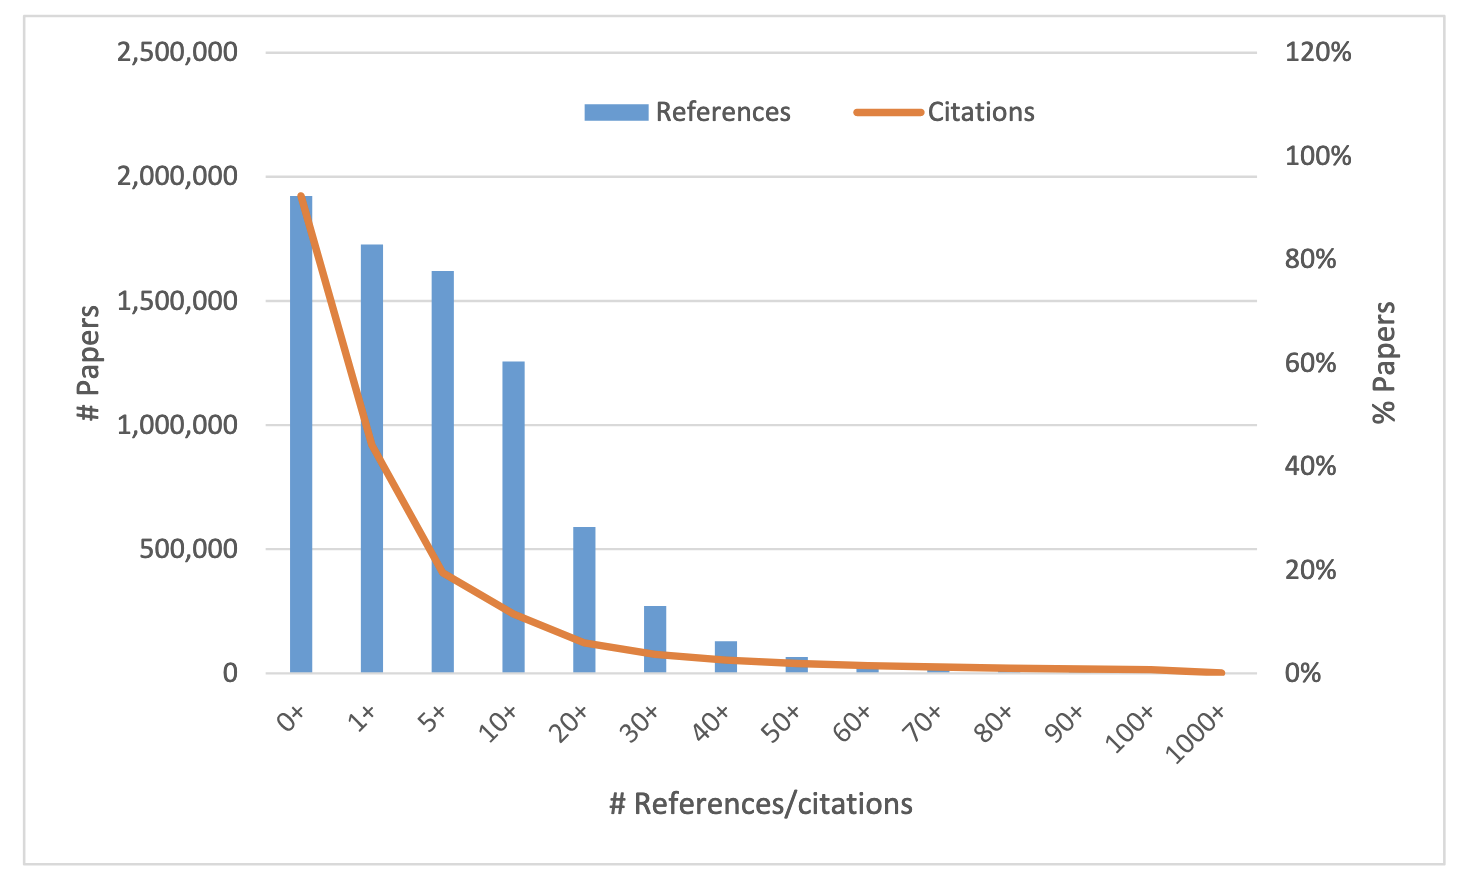
\includegraphics[scale=0.375]{figs/citations_per_paper.png}
		\caption{Distribuição do número de referências e citações por artigo~\cite{Fiala:17}.}
		\label{f.citations_per_paper}
	\end{figure}	
\end{frame}

\subsection{Por que investir?}
\label{ss.why_visibility}

\begin{frame}{Por que investir?}
	\justify 
	\begin{itemize}
		\item<1> Ampliar o alcance e o possível impacto social da pesquisa;
		\\~\\
		\item<2> ``Expor"~o nome da universidade em que a pesquisa foi conduzida;
		\\~\\
		\item<3> Possibilitar a colaboração com pesquisadores de outras universidades e centros de pesquisa;
		\\~\\
		\item<4> Mérito pessoal, aspirações profissionais, dentre outros.
	\end{itemize}
\end{frame}

\begin{frame}{}
	\centering
	\begin{figure}
		
\includegraphics[scale=0.2]{figs/keras.png}
		\caption{A biblioteca Keras~\cite{Chollet:15}, desenvolvida por François Chollet, foi incorporada ao Tensorflow e o autor contratado pela Google.}
		\label{f.keras}
	\end{figure}
\end{frame}


\subsection{Como ampliar?}
\label{ss.how_visibility}

\begin{frame}{Como ampliar?}
	\justify 
	\begin{itemize}
		\item Exposição de pré-publicação e/ou código aberto relacionado à pesquisa;
		\\~\\
		\item Documentação para terceiros conseguirem reproduzir a pesquisa;
		\\~\\
		\item Manutenção e disponibilidade para responder dúvidas e auxiliar usuários em utilizar a pesquisa;
		\\~\\
		\item Divulgação da pesquisa em redes sociais e/ou locais pertinentes.
	\end{itemize}
\end{frame}
\section{Comunidade acadêmica}
\label{s.community}

\begin{frame}{Comunidade acadêmica}
	\justify 
	\begin{itemize}
		\item<1> Grupo de pessoas de instituições de ensino superior as quais engajam-se em atividades ``intelectuais", tais como \textbf{ensino}, \textbf{aprendizado} e \textbf{pesquisa};
		\\~\\
		\item<2> Comunidade deve ser \textbf{inclusiva}, \textbf{diversa} e \textbf{abrangente}, não limitando a participação de quaisquer pessoas;
		\\~\\
		\item<3> Como garantir que as pesquisas sejam ``honestas"~e sigam um conjunto de \textbf{boas práticas}?
	\end{itemize}
\end{frame}

\begin{frame}{}
	\centering
	\begin{figure}
		
\includegraphics[scale=0.125]{figs/lead_country_papers.png}
		\caption{Ranking de países líderes em publicações nas áreas de Ciência e Engenharia no ano de 2018~\cite{Statista:18}.}
		\label{f.lead_country_papers}
	\end{figure}
\end{frame}

\subsection{Reprodutibilidade e integridade}
\label{ss.reproducibility_integrity}

\begin{frame}{Reprodutibilidade e integridade}
	\begin{block}{\centering Reprodutibilidade}
		Pesquisa deve ser passível de reprodução pela comunidade a partir da leitura do artigo e da utilização de ferramentas disponibilizadas.
	\end{block}
	\vspace{1cm}
	\begin{block}{\centering Integridade}
		Pesquisa deve ser íntegra, ou seja, os autores devem reportar honestamente o objetivo, metodologia e resultados obtidos.
	\end{block}
\end{frame}

\subsection{Impacto social}
\label{ss.social_impact}

\begin{frame}{Impacto social}
	\justify 
	\begin{itemize}
		\item<1> Existem \textbf{diversos fatores} que contribuem para o \textbf{``sucesso"}~de uma pesquisa;
		\\~\\
		\item<2> O processo de pesquisa \textbf{não} pode ser exclusivamente \textbf{dependente} de \textbf{métricas}, tais como, visibilidade, citações, dentre outras;
		\\~\\
		\item<3> \textbf{Inúmeras} pesquisas contribuem mais com \textbf{impactos sociais} do que com impactos acadêmicos.
	\end{itemize}
\end{frame}

\begin{frame}{}
	\centering
	\begin{figure}
		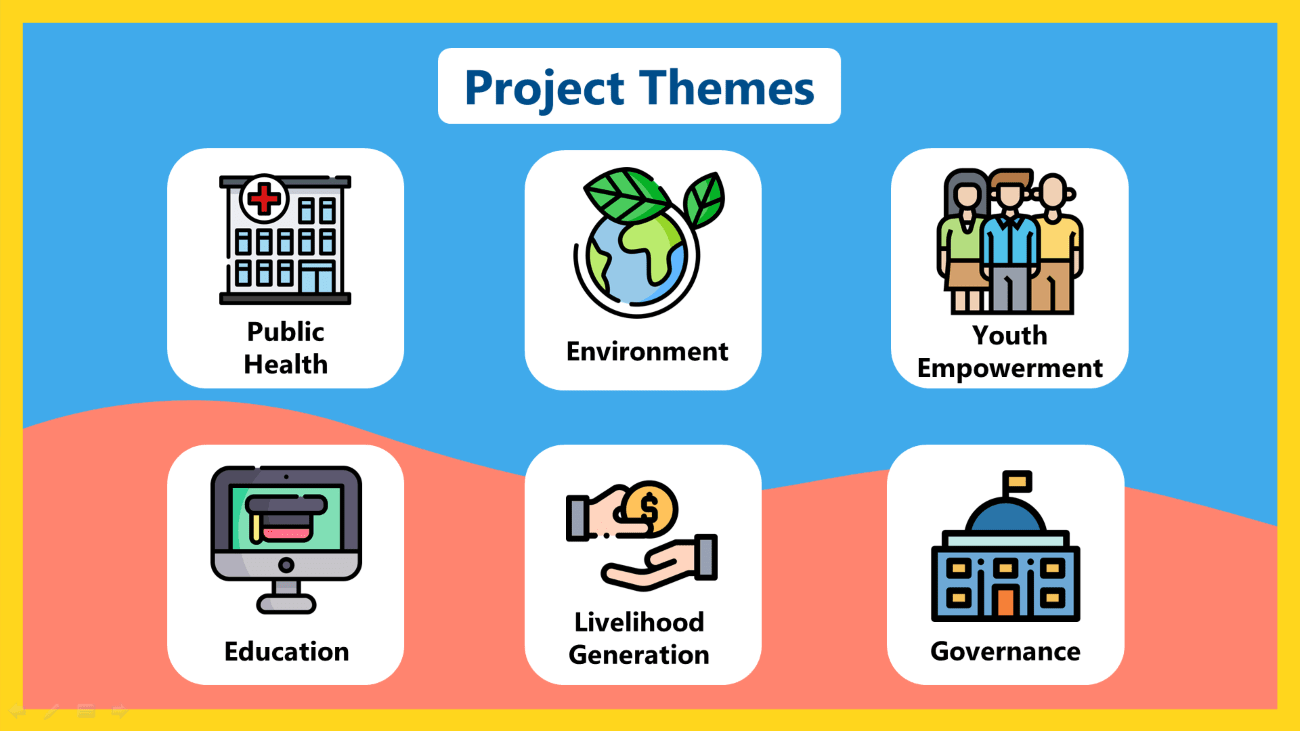
\includegraphics[scale=0.2]{figs/social_impact_research.png}
		\caption{Exemplos de áreas que beneficiam-se com o impacto social das pesquisas~\cite{YLAC:21}.}
		\label{f.social_impact_research}
	\end{figure}
\end{frame}

\section{Compartilhamento público}
\label{s.public_sharing}

\begin{frame}{Compartilhamento público}
\end{frame}

\subsection{Pré-publicação}
\label{ss.research}

\begin{frame}{Pré-publicação}
\end{frame}

\subsection{Código aberto}
\label{ss.integrity}

\begin{frame}{Código aberto}
\end{frame}

\subsection{Ferramentas gratuitas}
\label{ss.free_tools}

\begin{frame}{Ferramentas gratuitas}
\end{frame}

\section{Aplicação prática em Python}
\label{s.python_application}

\begin{frame}{Aplicação prática em Python}
	\justify 
	\begin{itemize}
		\item<1> O principal objetivo deste \textbf{tutorial} é construir uma \textbf{aplicação prática} em \textbf{Python};
		\\~\\
		\item<2> Aplicação será um \textbf{pacote/biblioteca}, hospedado no GitHub e compartilhado no repositório oficial PyPI;
		\\~\\
		\item<3> Pacote/biblioteca será composto por arquivos básicos para \textbf{instalação}, \textbf{dependências}, \textbf{documentação} e \textbf{testes unitários};
		\\~\\
		\item<4> Por fim, serão apresentados alguns exemplos de como \textbf{melhorar} a \textbf{divulgação} e \textbf{atrair} o uso da \textbf{comunidade}.
	\end{itemize}
\end{frame}

\subsection{Criação de repositório}
\label{ss.repository_creation}

\begin{frame}{Criação de repositório}
	\begin{figure}
		\centering
		
\includegraphics[scale=0.125]{figs/video_play.png}
	\end{figure}
\end{frame}

\subsection{Implementação}
\label{ss.implementation}

\begin{frame}{Implementação}
\end{frame}

\subsection{Submissão ao PyPI}
\label{ss.pypi_submission}

\begin{frame}{Submissão ao PyPI}
\end{frame}

\begin{frame}{}
	\begin{figure}
		\centering
		
\includegraphics[scale=0.125]{figs/video_play.png}
	\end{figure}
\end{frame}

\subsection{Locais de divulgação}
\label{ss.places_sharing}

\begin{frame}{Locais de divulgação}
\end{frame}
\section{Conclusão}
\label{s.conclusion}

\begin{frame}{Conclusão}
	\justify 
	\begin{itemize}
		\item<1> \textbf{Garantir} reprodutibilidade e integridade da pesquisa utilizando um conjunto \textbf{boas práticas};
		\\~\\
		\item<2> \textbf{Ampliar} a \textbf{visibilidade} através de pré-publicações, código aberto e apoio a comunidade;
		\\~\\
		\item<3> \textbf{Possibilitar impactos sociais} e \textbf{acadêmicos} ao aumentar a visibilidade da pesquisa;
		\\~\\
		\item<4> Fomentar \textbf{aprendizado contínuo} e melhorar as capacidades de produção de pesquisa.
	\end{itemize}
\end{frame}

% Defines the references and its slides
\section*{Referências}
\begin{frame}[allowframebreaks]
	\bibliography{references}
	\bibliographystyle{unsrt}
\end{frame}

% Defines the standout finishing slide
\begin{frame}[plain,standout]
	\vspace*{2cm}
	Perguntas?
	\\~\\
	Obrigado pela atenção!
	\\~\\
	\begin{figure}[!ht]
		\centering
		
\includegraphics[scale=0.1]{figs/recogna_clear.eps}	
	\end{figure}
\end{frame}

% Ends the document
\end{document}